\chapter{Global Methods}
\color{black}
\begin{comment}
\begin{blueshaded}
Structure du chapitre: 
\begin{itemize}
    \item[1] Neuron: modèle
    \item[2] Switches entre les modes
    \item[3] Circuits, courant synaptiques
    \item[4] Plasticité
    \item[5] Mesure et Analyses (LFP, spectrogramme)
\end{itemize}

\end{blueshaded}
\end{comment}



% -------------------------------
% -------------------------------
%
%     RESEARCH CONTEXT
%
% -------------------------------
% -------------------------------

\textcolor{red}{INTRO du chapitre}


\section{Neuron modeling}
Modeling the membrane voltage $V_\mathrm{m}$ by an equation is a crucial step in the quest of investigating the neuron activity and is therefore a fundamental component of this thesis. In this section, I present an overview of modeling and review the various types of models described in the literature to establish a foundational understanding of this subject matter.



% -----------------------------------
%       Basic knowledge
% -----------------------------------
\subsection{Modeling a neuron as an RC circuit with voltage-dependent ion channels}
A neuron is often described as an equivalent RC circuit. Its membrane is not permeable to ions, it acts as a capacitance defined by $C_\mathrm{m}$ producing a capacitance current $I_C$: 
$$I_C = C_\mathrm{m} \dot{V}_\mathrm{m}$$ 
The ion channels allow the flow of ion. The global activity of all the same ion channels are modeled as a conductance that is non-linearly dynamically regulated. The ion channels are often voltage-dependent, modeled by an voltage-dependent activation and inactivation gates. Ion flows through the channel following the concentration gradient until it reaches its ion reversal potential $E_i$. Altogether, the current flowing through the channel is described by the Ohm's law: $$I_{\mathrm{ion}} =  g_{\mathrm{ion}} (V_\mathrm{m} - E_{\mathrm{ion}})$$
where $E_{\mathrm{ion}}$ is the reversal potential also called Nernst potential and $g_\mathrm{ion}$ is the equivalent ion channel conductance. The conductance can vary between 0 when all the channels are closed up to the maximal conductance $\bar{g}_{\mathrm{ion}}$ when all the channels are open. The maximal conductance depends depends on the density of ion channel at the membrane. The opening and closing of the ion channels are regulated by activation and inactivation gates respectively modeled by $m_{\mathrm{ion}}$ is the activation variable and $h_{\mathrm{ion}}$ is the inactivation variable. And so the current flowing through an ion channel is 
$$I_{\mathrm{ion}} = \bar{g}_{\mathrm{ion}} m_{\mathrm{ion}}(V_\mathrm{m}) h_i(V_\mathrm{m}) (V_\mathrm{m} - E_i)$$

These gates are voltage-dependent and are governed by the following dynamics: 
$$ \tau_{x_{\mathrm{ion}}} (V_\mathrm{m}) \dot{x}_{\mathrm{ion}} = x_{{\mathrm{ion}},\infty}(V_\mathrm{m}) - x_{\mathrm{ion}}$$
where $x$ corresponds to either the activation or inactivation gate, $\tau_{x_{\mathrm{ion}}}$ is the voltage-dependent time-constant and $x_{{\mathrm{ion}},\infty(V_\mathrm{m})}$ is the voltage-dependent steady state value, which is the fraction of open ion channel at the steady state at a given value of $V_\mathrm{m}$. These two voltage-dependent variables are often defined by sigmoidal functions.  

Modeling neuron as a RC circuit with voltage-dependent conductance was a huge breakthrough in computational neuroscience brought by Hodgkin and Huxley seventy years ago \citep{hodgkin_quantitative_1952}. It provided a strong framework to simulate an action potential, through the interaction between sodium and potassium channels that are activated at different timescales and values of the membrane potential. This interplay is embedded in the different equations describing the time constants and the gating variables of the different ion channels. These equations were fitted on electrophysiological recordings. 

Altogether,  Kirchoff's current law is applied on the capacitance current, the sum of all the ion currents and the external applied current $I_{\mathrm{app}}$
$$I_C + \sum_i I_{\mathrm{ion}} + I_{\mathrm{app}} = 0$$
Finally, the evolution of the membrane potential is defined by
\begin{equation}
 C_\mathrm{m} \dot{V}_\mathrm{m} = \sum_i I_{\mathrm{ion}} + I_{\mathrm{app}} 
 \label{eq:HH}
 \end{equation}

\begin{minipage}{0.45\textwidth}
This framework has been extensively used over the past few decades. Like any model, it has its advantages and disadvantages. Each ion channel is described by one or two differential equations for the gates, which significantly increases the computing time but offers valuable biophysical insights. The various parameters have to be fitted according to the region, which presents a challenging degree of freedom \citep{prinz_alternative_2003}. 
\textcolor{gray}{For this thesis, I have opted to use this framework as it provides a dependable description of the neuron's behavior, and I avoid oversimplifying the dynamics. --- à ajouter fin de la section}

\end{minipage}
\hfill
\begin{minipage}{0.45\textwidth}
    \begin{lilashaded}
        Fun fact sur la première simulation de HH (durée, ordinateur, ...) 
    \end{lilashaded}
\end{minipage}



% -----------------------------------
%       List of neuron models
% -----------------------------------

\subsection{Describing Neuron Spiking Activity}
\subsubsection{From Biophysical to Abstract Models}
The conductance-based model offers a detailed framework for accurately predicting the evolution of the membrane voltage. However, if one is only interested in spike timings, using this model can be computationally expensive. The choice of an appropriate neuron model depends on the application, research question, and desired level of detail.

This section presents a non-exhaustive list of computational models used to describe neuron activity, divided into five categories: conductance-based model, integrate-and-fire model, event-based model, rate-based model and more complex models grouped under the category of 'Others'. For further details, refer to \citep{gerstner_neuronal_2014}.



\begin{itemize}
\item \textcolor{blue}{Conductance-based model (Cond)}\\ 
The voltage of the neuron's membrane, denoted as $V_\mathrm{m}$, can be described using the Hodgkin and Huxley formalism \citep{hodgkin_quantitative_1952} as shown in equation~\eqref{eq:HH}. The number of ion channels present in the neuron depends on its type and location and can be modeled as a single-point neuron or as multiple compartmental models. The timing of a neuron's spike can be determined by tracking the point at which its membrane voltage crosses a certain threshold.
\item \textcolor{blue}{\acrfull{IF}} \\
This implementation aims to describe the shape of the action potential until it reaches its threshold, also called the subthreshold dynamics and it skips the detail concerning the fast increase of the membrane voltage. It lies on the equivalence of the RC circuit by modeling the charge of a capacitance. Its generic equations is
$$ C_\mathrm{m} \dot{V}_\mathrm{m} = - g_{leak} (V-E_{leak}) + I_{\mathrm{app}} \mbox{\hspace{2cm} if } V_\mathrm{m} = V_{\mathrm{th}} \mbox{, then } V = V_{\mathrm{rest}} $$
where $g_{\mathrm{leak}}$ is the fixed ohmic leak conductance to account  for all ion channels, $E_{\mathrm{leak}}$ Nernst potential. For a sufficient applied current $I_{\mathrm{app}}$, the membrane potential $V_\mathrm{m}$ increases until a threshold value $V_{\mathrm{th}}$. Then, it is reset to the resting state $V_{\mathrm{rest}}$. The potential increases again until the reset and so on. There are several types of \acrshort{IF} models detailed in [\cite{gerstner_neuronal_2014}]. This formulation is faster compared to conductance-based model but lacks of biological details. Variations of \acrshort{IF} are encountered in computational models such as the \acrfull{QIF} or \acrfull{AdEx} among others.
\item \textcolor{blue}{Event-based (EB)}\\
The membrane voltage is not explicitly or as precisely described as in a conductance-based model or in an \acrshort{IF} model. The spike timing activity is given as a \textit{train of spikes}. Computationally, it can be a simple vector of time associated to each spike time. It is directly injected through a term $\delta(t-t_{\mathrm{spk}})$. The simulation only uses the spike trains to drive its model. 
\item \textcolor{blue}{Rate-based}\\
The governing equation is: 
$$ \tau \dot{r} = - r + F(I)$$
where $\tau$ is the decay timeconstant, $r$ is the rate of the neuron in Hz and $F(I)$ is the function the input current. It assumes that the activity of the neuron can be described by its average firing rate. It is simpler than \acrshort{IF}. It is often used in large-scale model.
\item \textcolor{blue}{Others}\\
This category gathers diverse models such as multiple-timescale adaptable model with threshold [\cite{lappalainen_theoretical_2019}], model considering only \acrfull{BPAP}, \acrshort{EPSP} or models converting spike time into exponential decaying term to mimic the membrane voltage fluctuation. More biological details can be added to deliver an equation of the neuron activity. Therefore, this category permits to encapsulate models that are not perfectly following the more common design of conductance-based model, \acrshort{IF}, event-based implementation.
\end{itemize}

\textcolor{red}{MONTRER une image recap des différentes implémentations depuis la litérature }

\subsubsection{Using dynamical systems analysis}
In the previous section, I provided models that describe the firing of action potentials. However, the conductance-based model, for instance, is defined by a large number of differential equations. Understanding how the model operates through analytical development is nearly impossible, leaving us only with simulations. However, non-linear systems analysis offers an attractive solution to overcome simulation and directly study the dynamics. Phase plane and bifurcation analyses can unveil meaningful understanding of the models. APPENDIX \textcolor{red}{XXXXX} provides a tutorial of introduction in non-linear system analysis. 

To use these tools, it is necessary to reduce the model's dimensionality. The common practice is to aggregate different variables based on their fast, slow, and ultraslow dynamics. The fast variables are considered at their steady-state value, and the slow variables are aggregated into a single slow variable. Another systematic way to reduce the number of equations is to decompose each variable into a weighted sum at different timescales. This technique is known as \acrfull{DIC} \citep{drion_dynamic_2015}.

~\\
\citep{franci_organizing_2012,franci_balance_2013} "understanding excitability in detailed conductance-based models remains a challenge, especially for neurons that exhibit transition between distinctively different firing types depending on environmental conditions" -- via les PP + bifurcations, Franci can characterize the different neuronal firing patterns. 

\begin{pinkshaded}
\textcolor{red}{Image: \\
Montrer un plan de phase du H-H et le réduire et expliquer le portrait de phase. }
~\\
\textcolor{blue}{Expliquer l'apparition de la branche du bas sur le portrait de phase (...) pourquoi pour plus tard introduire la notion de switch entre tonic et burst}
\end{pinkshaded}




\subsection{Mathematical analysis of neuron model}
Neuron membrane potential is often described with a system of non-linear differential equations, that makes the analysis and the understanding a challenging task. For example the first conductance-based model established 70 years ago by Hodgkin and Huxley contains four differential equations.  Reducing their dimensionality is nice solution to study their dynamics with mathematical tools such as the phase plane analysis. 


\color{gray}
% -----------------------------------
%       PP tool
% -----------------------------------
---- aller voi l'appendix


% -----------------------------------
%       Model reduction
% -----------------------------------
\subsection{Model reduction}
The well-known \acrshort{HH} model is a good starting point to introduce model reduction and uncover the dynamics of the membrane potential in a phase plane. 

\textcolor{orange}{\textbf{EST-CE QUE c'est vraiment utile ?} }

$\bullet$ montrer l'exemple de HH et dire qu'on voit apparaitre une nullcline N-shape cubique et soit une sigmoide soit une droite. \\
$\bullet$ introduire les modeles plus "math" qui se sont simplement dit on va reproduire l'allure cubique. Il y a meme des modèles qui vont encore plus loin et qui ne reprennent que la parabole et la droite et utilise un système de reset pour avoir les spikes (izh, vanpottelbergh...) \\
$\bullet$ expliquer les réductions de modèles sont utiles mais il faut faire attention à 'get rid off' des bonnes informations ... et du coup une nouvelle manière de faire c'est d'utiliser les DIC pour conserver les dynamics à différentes échelles de temps des canaux ioniques. \\


% -----------------------------------
%       PP of neuron
% -----------------------------------
\subsubsection{Phase plane analysis in a reduced neuron model}


% -----------------------------------
%       Bursting
% -----------------------------------

\subsection{The phase portrait of the switch from tonic firing to bursting}


\textcolor{blue}{Reduced models}\\
The \acrshort{HH} formalism has a large amount of differential equations that is time and energy consuming to run on computers. 
\textcolor{blue}{est-ce que l'on met ici ou dans le tools neuroscience }
(tout ce qui est utile pour l'article de Plos 2021)

\color{black}




% -------------------------------
%     Modeling switches
% -------------------------------

\subsection{Modeling switches from tonic firing to bursting}
The previous section have depicted an image of the neuron modeling. In my thesis, I investigate the switch from tonic spiking to bursting. Several methods can be used to induce a switch from tonic to burst:


To model the transitions between wake and sleep states the model included synaptic and intrinsic mechanisms which reflect the changes in neuromodulatory tone during these different arousal states \citep{gonzalez_can_2020}


change in synaptic weight : \citep{capone_sleep-like_2019} weights between inhibitory and excitatory neurons in the cortex is reduced." + change in intrisinc parameter in adEX model (math param).

Hill tonic to burst: increasing the potassium leak conductance gKL (from 1.0 to 1.85), -- mimic reduced actin of Ach during sleep + est that muscarinic receptor activation can significantly inhibit the INa(p) conductance

he removal of acetylcholine would therefore cause an effective increase in the conductance of INa(p) throughout the network. We model this by increasing the conductance gNa(p) for the sleep mode (from 0.5 to 1.25). Acetylcholine has also been shown to shift the activation curve of Ih to more depolarized levels

We model this by increasing the conductance of Ih during the sleep mode (from 1.0 to 2.0

We model this by increasing the peak conductance of IT from wakefulness to sleep (from 1.0 to 1.25).

e increased gDK (from 0.5 to 1.25) i

We model this change by increasing the amplitude of AMPA EPSPs (by 50%) from the waking mode to the sleep mod

increasing K out (\citep{bacak_modeling_2016}. 


\begin{itemize}
    \item Conductance-based: change in the ion channel conductance, change in K+ concentration, hyperpolarization.
    \item IF: \textcolor{red}{lire BTDP de julijana} + \citep{van_pottelbergh_robust_2018}
    \item Mathematical models: \\
    "a fast time-scale for the spike generation, a slow time-scale for the intraburst spike frequency, and an ultraslow time-scale for the interburst frequency. "\citep{franci_modeling_2014}
\end{itemize}

\color{gray}


Examples in the literature: \\
- \citep{rasmussen_chaotic_2017}: models of average-neuron able to switch from sleep- quiet wakefulness and active wakefulness. \\
- \citep{esser_breakdown_2009, krishnan_cellular_2016} boucle TC machin avec enregistrement cellulars, LFP et spectrogram. \\
- \citep{wang_neurophysiological_2010} looong paper/review of cortical rhythms for cognition with models and synchronisation (focus on E-I).

\begin{comment}
\begin{figure}[h!]
    \centering
    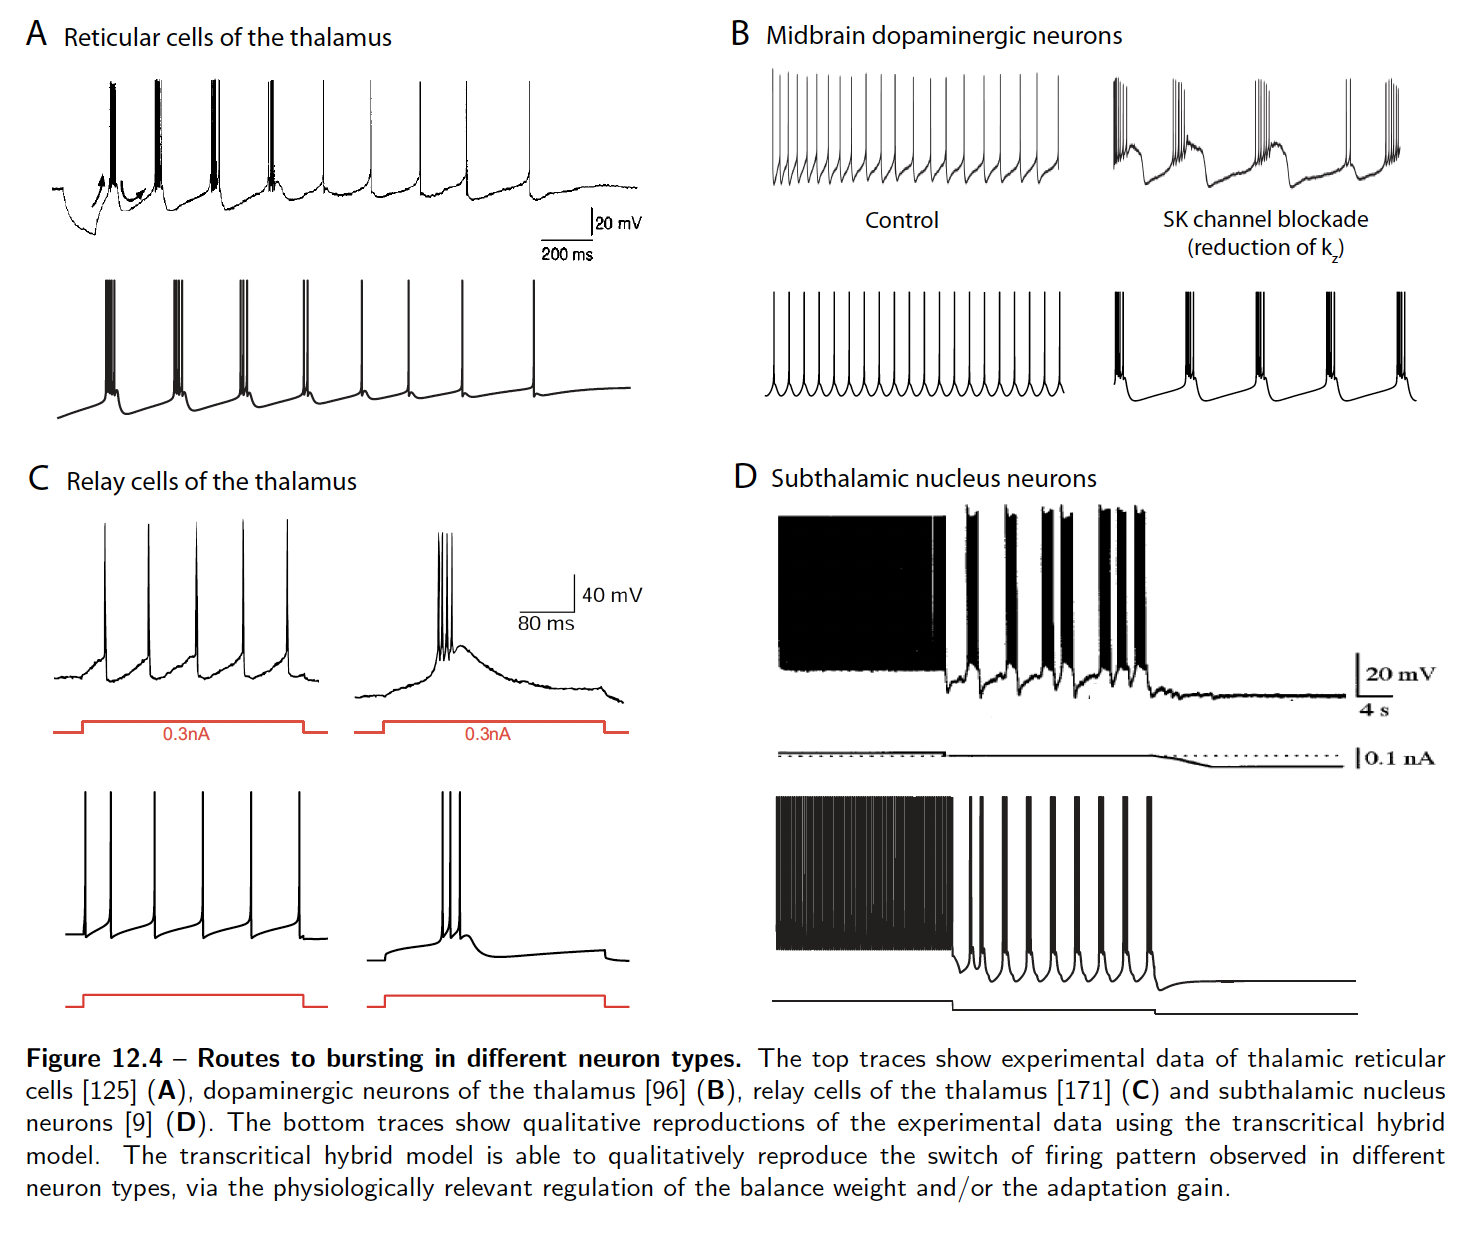
\includegraphics[scale=0.4]{latex/fig/Methods/GD_Thesis_Bursting.png}
    \caption{ ....}
    \label{fig:GD_Thesis_Bursting}
\end{figure}
\color{black}
\end{comment}


\color{black}
\subsection{The neuron model implemented in the context of this thesis}

\textcolor{red}{montrer une simu du modèle qui switch}

% -------------------------------
% -------------------------------
%
%     Circuit
%
% -------------------------------
% -------------------------------

\section{Circuit and network architecture}
Connecting neurons with each other is very easy following the electrical circuit equivalence of the neuron. Synaptic currents are simply modelled as input current:
$$ C_\mathrm{m}\dot{V}_\mathrm{m} = -\sum_i I_{\mathrm{ion},i} + I_{\mathrm{app}} + I_{\mathrm{syn}}.$$ 

In this thesis we consider four synaptic currents due to different postsynaptic receptors: \acrshort{AMPA}, \acrshort{GABA}\textsubscript{A} and \acrshort{GABA}\textsubscript{B}.

There are different manners to describe synaptic currents (see \citep{destexhe_circuit_2004}). In my thesis, I follow the \acrshort{HH} formalism such that the postsynaptic receptors allow flow of ions following the gradient concentration when the channel gate is open. The synaptic currents are defined by:
\begin{align*}
    I_{\mathrm{AMPA}}	&  = \bar{g}_{\mathrm{AMPA}} s_\mathrm{AMPA}(V_\mathrm{m} - 0) \\
    I_{\mathrm{GABA}_\mathrm{A}} &  = \bar{g}_{\mathrm{GABA}_\mathrm{A}}  s_{\mathrm{GABA}_\mathrm{A}} (V_\mathrm{m}-E_\mathrm{Cl})\\
    I_{\mathrm{GABA}_\mathrm{B}}   &= \bar{g}_{\mathrm{GABA}_\mathrm{B}} s_{\mathrm{GABA}_\mathrm{B}} (V_\mathrm{m}-E_\mathrm{K})
\end{align*}
where $\bar{g}_{\mathrm{AMPA}}$,  $\bar{g}_{\mathrm{GABA}_\mathrm{A}}$ and $\bar{g}_{\mathrm{GABA}_\mathrm{B}}$ are the synaptic conductances. \\
~\\
\textcolor{magenta}{ATTENTION ETRE COHERENT DANS la rédaction du mécanisme de plasticité et des notations. Latter $\bar{g}_{\mathrm{AMPA}}$ is multiplied by the synaptic weight $w$ (see Plasticity implementation).}


AMPA receptor reversal potential is set to \SI{0}{\milli\volt}, GABA\textsubscript{A} receptor reversal potential is set to chloride reversal potential ($E_\mathrm{Cl} = \SI{-70}{\milli\volt}$) and GABA\textsubscript{B}  receptor reversal potential is set to potassium reversal potential ($E_\mathrm{K} = \SI{-85}{\milli\volt}$).

The gating variables of the synaptic receptors are $s_\mathrm{AMPA}$, $s_{\mathrm{GABA}_\mathrm{A}}$ and $s_{\mathrm{GABA}_\mathrm{B}}$ are variables whose dynamics depend on the activity of the presynaptic neuron. As the presynaptic neuron spikes, it releases neurotransmitters that bind to the receptors and open the receptors. To shortcup all the biological reactions, the gating variable dynamics is simply governed by the presynaptic activity. In my thesis, I use the presynaptic membrane potential:
\begin{align*}
	\dot{s}_\mathrm{AMPA} & = 1.1 \, T_\mathrm{m} (1-s_\mathrm{AMPA}) - 0.19 \,s_\mathrm{AMPA} \\
	\dot{s}_{\mathrm{GABA}_\mathrm{A}} &= 0.53 \, T_\mathrm{m} (1- s_{\mathrm{GABA}_\mathrm{A}}) - 0.18 \,s_{\mathrm{GABA}_\mathrm{A}} \\
	\dot{s}_{\mathrm{GABA}_\mathrm{B}} &= 0.016 \, T_\mathrm{m} (1- s_{\mathrm{GABA}_\mathrm{B}}) - 0.0047\, s_{\mathrm{GABA}_\mathrm{B}}
\end{align*}
with transmitter concentration $T_\mathrm{m}$ depends on the presynaptic membrane voltage and the dynamics follows the formalism described in \cite{destexhe_synthesis_1994}, that is,
$$T_\mathrm{m}(V) = \dfrac{1}{1+\exp\left[-(V-2)/5\right]}.$$ 
The numerical values (1.1, 0.19, 0.53, 0.18, 0.016 and 0.0047) are rate parameters to mimic the kinetics of the synaptic receptors. These values originated from \cite{destexhe_synthesis_1994}. The smallest, the slowest the kinetics. For GABA\textsubscript{B}, the kinetics is slower which is coherent with the metabotropic nature of this receptor. Other models of synaptic receptor gating variables use the presynaptic spike time is integrated over time \textcolor{red}{REF}.

The synaptic current through \acrshort{NMDAr} requires an additional term modeling the effect of the magnesium blocker: 
$$ I_{\mathrm{NMDA}}	= \bar{g}_{\mathrm{NMDA}} B(V_\mathrm{m}) s_\mathrm{AMPA}(V_\mathrm{m} - 0) $$
where $B(V_\mathrm{m})$ is a sigmoidal function dependent on the postsynaptic membrane potential. For the purpose of this thesis, I follow the implementation of \citep{graupner_calcium-based_2012} to ease the implementation of synaptic plasticity \textcolor{red}{SEE SECTION}. 


\textcolor{blue}{jutifier le choix du réseau:} \citep{sherman_functional_1996}.\\

\textcolor{red}{expliquer que les courants synaptiques ne vont pas seulement utiliser V mais peuvent aussi utiliser les spikes times etc voir Destexhe 2004}


\subsection{Circuit used in the context of this thesis}
\textcolor{red}{montrer une simu d'un petit circuit à trois neurones}

~\\
\newpage

% -------------------------------
% -------------------------------
%
%            PLASTICITY
%
% -------------------------------
% -------------------------------

\section{Synaptic plasticity}
As described in the previous chapter, neurons have the ability to change their connections with each other based on their activities. Modeling synaptic plasticity consists in creating a model seen as a black box, that uses the pre- and postsynaptic activities as inputs and provided the synaptic strength as output. It is a challenging task because it requires several model decisions, called model features,  such as the choice of the region of interest, the network size, the neuron model and the definition of the synaptic strength. Then, the core of the challenge is to create the dynamics that governs the evolution of the synaptic strength, namely the synaptic plasticity rule itself. 

\textcolor{magenta}{etre rigoureuse dans la def de w partout}
%In the following section, I explain the diverse computational model features often encountered in the literature. 


\begin{figure}[h!]
    \centering
    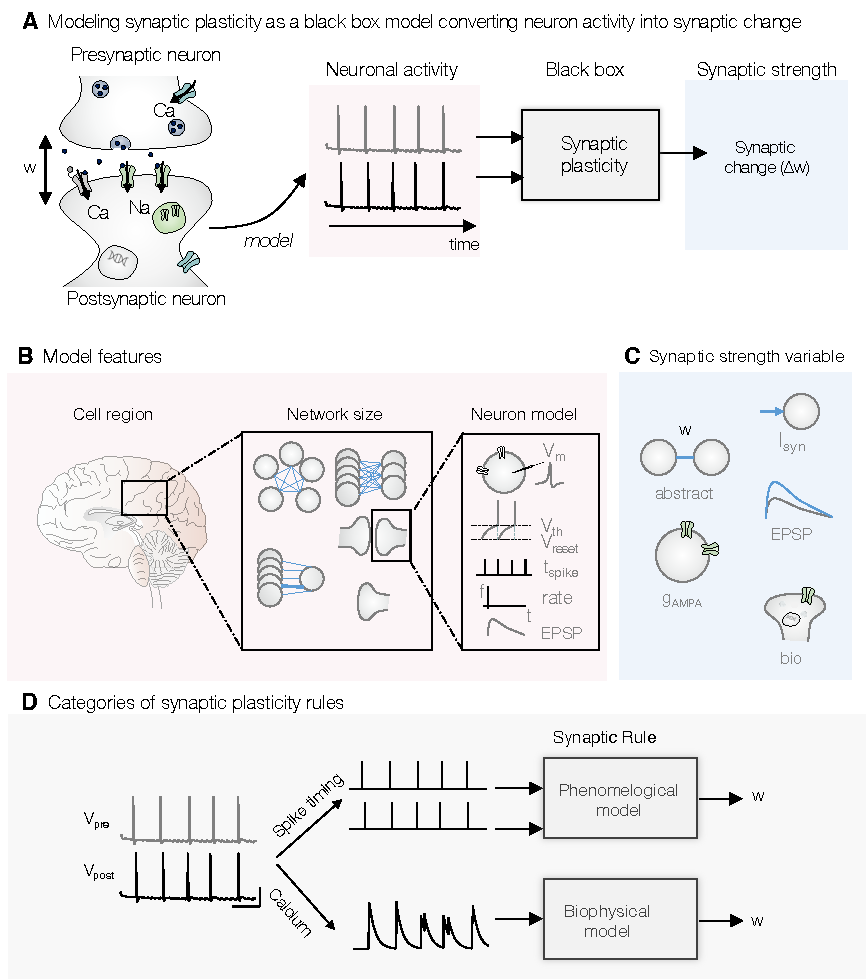
\includegraphics[scale=1]{fig/Methods/FeaturesRecap.pdf}
    \caption{Cpation}
    \label{fig:Methods_FeaturesRacap}
\end{figure}

\begin{comment}
    OLD CAPTION

    \caption{\textbf{A.} \textbf{Model features shared in computational models of synaptic plasticity rule}. \textit{Cell region}: plasticity can be explored in different neuron types located such as hippocampus, cortex, striatum or thalamus. The neuron parameters can be adapted to mimic different neuron types or one can use an abstract neuron. \textit{Network size}: plasticity can be studied in a network composed of several neurons or formed in assembly shape, between several presynaptic neurons projecting to one postsynaptic neuron, between a pre- and post-synaptic neuron or at the postsynaptic level. \textit{Neuron model}: the neuron follows a conductance-based model (with a membrane voltage Vm) or an \acrfull{IF} formalism. Only the spike trains or the firing rate is considered, or another principle is used such as the \acrshort{EPSP} or more complex neuron shape. \textit{Synaptic strength}: the weight is abstract and does not influence the rest (w, top-left scheme), the weight directly influences the synaptic input, the change in synaptic transmission is quantified by the change in \acrshort{EPSP} (top-right scheme), the change of \acrshort{AMPAr} is measured (bottom-left scheme) or the weight is measured by more biological quantities (bottom-right scheme).\\
    \textbf{B.} The synaptic weight $w$ change is governed by the neuronal activity thanks to phenomenological models (top) (written as phenom.) or by calcium thanks to biological models (bottom). \textcolor{red}{ajuster les couleurs avec les couleurs du rappel}}
    
\end{comment}

% -----------------------------------
%
%             SP (features)
%
% -----------------------------------

\subsection{Model features}
%Figure \ref{fig:Review_blackbox}A 
Table \textcolor{red}{XXX} gathers the different network and neuron features. 

% -----------------------------------
%       SP (features): neurons modeling choice
% -----------------------------------
\subsubsection{The region of interest}
First of all, synaptic plasticity varies depending on the brain \textit{region}. It has been commonly modeled for neurons in the hippocampus \citep{abarbanel_biophysical_2003, van_rossum_stable_2000}, the cortex \citep{chen_heterosynaptic_2013}, the striatum \citep{nakano_kinetic_2010, jedrzejewska-szmek_calcium_2017} or the thalamus \citep{gjorgjieva_burst-time-dependent_2009}. But thanks the freedom in computational models, a neuron can be adaptable by changing its parameters as done in \citep{graupner_calcium-based_2012, clopath_connectivity_2010} or we can encounter the notion of 'abstract neuron' meaning that the region or the type is not accurately defined and the parameters have been not fitted on experimental data. It is useful to study more general phenomenons or to study plasticity using the spike train only for example \citep{karmarkar_model_2002, liu_effects_2015} (it is correlated with the feature neuron modeling). 

% -----------------------------------
%       SP (features): network size
% -----------------------------------
\subsubsection{The network size}
The second feature is the \textit{network size}. Plasticity can be studied locally by considering only the postsynaptic site \citep{graupner_calcium-based_2012} or at the interconnection between a pre- and a postsynaptic neuron [...]. It is also common to see a large amount of presynaptic neurons projecting to a postsynaptic neuron \citep{chen_heterosynaptic_2013, gonzalez-rueda_activity-dependent_2018}. Thanks to the computer efficiency improvement, the network size can be increased from small networks of 10 neurons to very large network of thousands neurons [...]. Finally, memory engrams rise interest and can be studied in interconnected network \citep{delamare_intrinsic_2022}.




% -----------------------------------
%       SP (features): neurons modeling choice
% -----------------------------------
\subsubsection{Neuron modeling}
The third important feature is the computational model of the neuron, which must accurately reproduce its electrical activity. The most commonly used models include the \textit{conductance-based model (cond)}   \citep{hartley_understanding_2006, gerkin_phenomenological_2010}, the \textit{integrate-and-fire (IF)} model and its derivatives \citep{bush_calcium_2012, izhikevich_solving_2007}, the \textit{event-based} model   (event)\citep{shouval_converging_2002}, and \textit{rate-based} (rate) models \citep{delamare_intrinsic_2022}. More complex implementations, such as the description of the \acrfull{BPAP} and the \acrfull{EPSP}, have been developed, among others \citep{kumar_frequency-dependent_2011}. Although there are many other computational models of neuron activity, I will limit the discussion to these five approaches (as defined in \textcolor{red}{SECTION XXX}. For further information, refer to \citep{gerstner_neuronal_2014}.



% -----------------------------------
%       SP: calcium modeling
% -----------------------------------
\subsubsection{Calcium modeling}
 Calcium is often used as the key driver to induce synaptic change. The correspondence between the change in calcium and the related pre- and postsynaptic spiking is implemented in several manners. Here, I list some common modeling practices (see Table \ref{tab:calcium features}). First, the \textit{calcium source} must be explicit such as NMDAr or voltage dependent calcium channels (VDCC) [..]. It can also come from more complex mechanisms such as intracellular stores such as endoplasmic reticulum \citep{berridge_neuronal_1998, jaeger_spike_2014}. Calcium is also released via activation of metabotropic glutamate receptors. Others calcium-dependent mechanisms can be integrated such as calcium-extrusion mechanisms, including membrane pumps, intake and uptake into intracellular calcium-stores. Or by contrast, calcium can be abstract and explicitly described by a mathematical variable directly translating the neuronal activity without intermediate terms [...].  Second, calcium from NMDAr is frequently used, the \textit{description of NMDAr} is also various. It can be expressed by a simple synaptic variable equation [...], a more complex detailed equations of its kinetics [...] or relatively simple by converting the spike timing activity \citep{jaeger_spike_2014}. Finally, the \textit{calcium dynamics} provides the time-evolution of the calcium that is affecting the synaptic strength. Several descriptions exist. For example, a differential equation converts the calcium from NMDAr or NMDAr and VDCC into a calcium fluctuation [...]. Once again, its dynamics can be also expressed very abstractly [...] or with a lot of intermediate terms to mimic the whole complex process [...].


Table \ref{tab:calcium features} provides the overview of the different calcium modeling practices. Conceptual equations are presented. Each article might adapt the equation form for example by adding scaling factors. 
\\


\begin{table}[H]
\begin{small}
    \centering
    %\resizebox{\textwidth}{!}{%
    \begin{tabular}{lll}
    \hline
    Feature & Notation & Description \\
    \hline
    Calcium source     &  &\\
        &  $ I_{\mathrm{NMDA}}$ & 
        \begin{tabular}[l]{@{}l@{}}
        $I_{\mathrm{NMDA}} = g_{\mathrm{NMDA}} s_{\mathrm{NMDA}} B(V_{\mathrm{post}}) (V_{\mathrm{post}} - E_{\mathrm{NMDA}})$ \\ 
        $g_{\mathrm{NMDA}}$: NMDA conductance\\
        $s_{\mathrm{NMDA}}$: gating variable \\
        $B(V_{\mathrm{post}})$ :  ... \end{tabular}\\
        &  $ I_{\mathrm{NMDA}} + I_{\mathrm{VDCC}} $ & ...\\
        & Others & eg: buffers, diffusion terms, pumps, ... \\
        &  $ \mbox{NMDA}(t_{\mathrm{spk}}) $ & Decreasing exponential at each postsynaptic spikes. \\
    \hline
    NMDA model   &   & \\  
        & Time   & Pre- or postsynaptic spike times govern the NMDA equation \\
        & Voltage & Pre- and postsynaptic voltages govern the NMDA equation \\
        & Kinetics & NMDAr is described by kinetic equations \\
        & / & No biological current\\
        & Others & More complex process describe the NMDAr \\
    \hline
    Calcium dynamics & &  \\
        & NMDA & 
        \begin{tabular}[l]{@{}l@{}}
        $\tau_{\mathrm{Ca}} \dot{\mathrm{Ca}} = \alpha I_{\mathrm{NMDA}} - \mathrm{Ca}$ \\
        $\alpha$: current-to-concentration factor
        \end{tabular} \\
        & NMDA + VDCC & \begin{tabular}[l]{@{}l@{}}
        $\tau_{\mathrm{Ca}} \dot{\mathrm{Ca}} = (\alpha I_{\mathrm{NMDA}} + \beta I_{\mathrm{VDCC}}) - \mathrm{Ca}$ \\
        $\alpha, \beta$: current-to-concentration factors
        \end{tabular}\\
        & $\delta (t_{\mathrm{spk}})$ & Simplified equation converting spike times into calcium variation\\
        & Others / Process & More biophysical description of the calcium change  \\
    \hline
    \end{tabular}
    %}
    \end{small}
    \caption{\textbf{Model features used to implement calcium in a neuron model}. There are various sources of calcium that can be considered. The implementation of the NMDA receptor dynamics varies between model. Calcium dynamics can be governed by calcium current sources or more abstract translating spike time activity. \textcolor{red}{Décider si on explique les équations dans le tableau ou non ? } }
    \label{tab:calcium features}
\end{table}


% -----------------------------------
%       SP: definition in models
% -----------------------------------
\subsubsection{The definition of the synaptic strength}
The last feature is the \textit{definition of the synaptic strength $w$} (see Figure~\ref{fig:Methods_FeaturesRacap}C) . I highlight five widespread forms. 
\begin{itemize}
\item \textcolor{blue}{Abstract}\\
The weight $w$ is simply a variable updated by the synaptic plasticity rule and it is not interfering in other model equations. It is encountered in more theoretical papers. I call it an abstract definition \textcolor{red}{REF}. 
\item \textcolor{blue}{$I_{syn}$}\\
The term $w$ is present in the model and weights the synaptic input. In an Integrate-and-Fire model or in a conductance based model,  the synaptic current is written $I_{\mathrm{syn}} = w F_{\mathrm{syn}}$ where $F_{\mathrm{syn}}$ either a function of the spiking time $\delta(t_{\mathrm{spk}})$ or pre- or postsynaptic membrane voltage $I_{\mathrm{syn}} = \bar{g}_{\mathrm{syn}}(V-E_{\mathrm{syn}}) $ such as  $\bar{g}_\mathrm{syn} = w \bar{g}_{syn}$ (resp. $w \bar{g}_{\mathrm{AMPA}}, w \bar{g}_{\mathrm{NMDA}}$). In more mathematical models, it weights the synaptic activity as done in \citep{tetzlaff_synaptic_2013}.
\item \textcolor{blue}{$g_{AMPA}$}\\ 
The synaptic strength directly refers to the conductance of the AMPA receptors. It translated the increase in efficacy or number of AMPA receptors. The differential equation governing the conductance change is driven by the activity of pre- and post-synaptic neurons ($A_{\mathrm{pre}}$ and $A_{\mathrm{post}}$) \citep{berridge_calcium_2014}:
\[ \dot{g}_\mathrm{AMPA} = F(A_{\mathrm{pre}}, A_{\mathrm{post}})\]
\item \textcolor{blue}{Bio}\\
The strength is quantified by biological quantities, for example the change in the concentration of phosphorylated \acrshort{CaMKII} or the concentration of active and phosphorylated AMPAr \textcolor{red}{REF}.
\item \textcolor{blue}{EPSP}\\
As done in experiment, the change in synaptic strength is measured by the change in the \acrshort{EPSP} before and after the induction protocol.
\end{itemize}




% -----------------------------------
%       SP: black box
% -----------------------------------
\subsection{Traditional synaptic plasticity rules}
Modeling of synaptic plasticity
%, neuronal activity and neuromodulation 
is trendy these recent years. Browsing the literature to find a synaptic rule adapted to your research can be very challenging. The number of publications providing models of synaptic rules is increasing with years. The rules can be declined following a very abstract equation to a huge set of detailed plasticity signaling reactions. A myriad of reviews detail models of synaptic plasticity rules since the last 20 years \citep{morrison_phenomenological_2008, citri_synaptic_2008, feldman_spike-timing_2012, feldman_spike_2020, shouval_models_2007, sjostrom_spike-timing_2010, manninen_postsynaptic_2010, lisman_questions_2010, markram_history_2011, markram_spike-timing-dependent_2012, van_rossum_computational_2013, fusi_limits_2007, senn_spike-timing-dependent_2020, magee_synaptic_2020, chrol-cannon_computational_2014}. In the following section, I recall the notion of synaptic plasticity rule and I explain the most encountered models.


\begin{comment}
\begin{figure}[H]
    \centering
    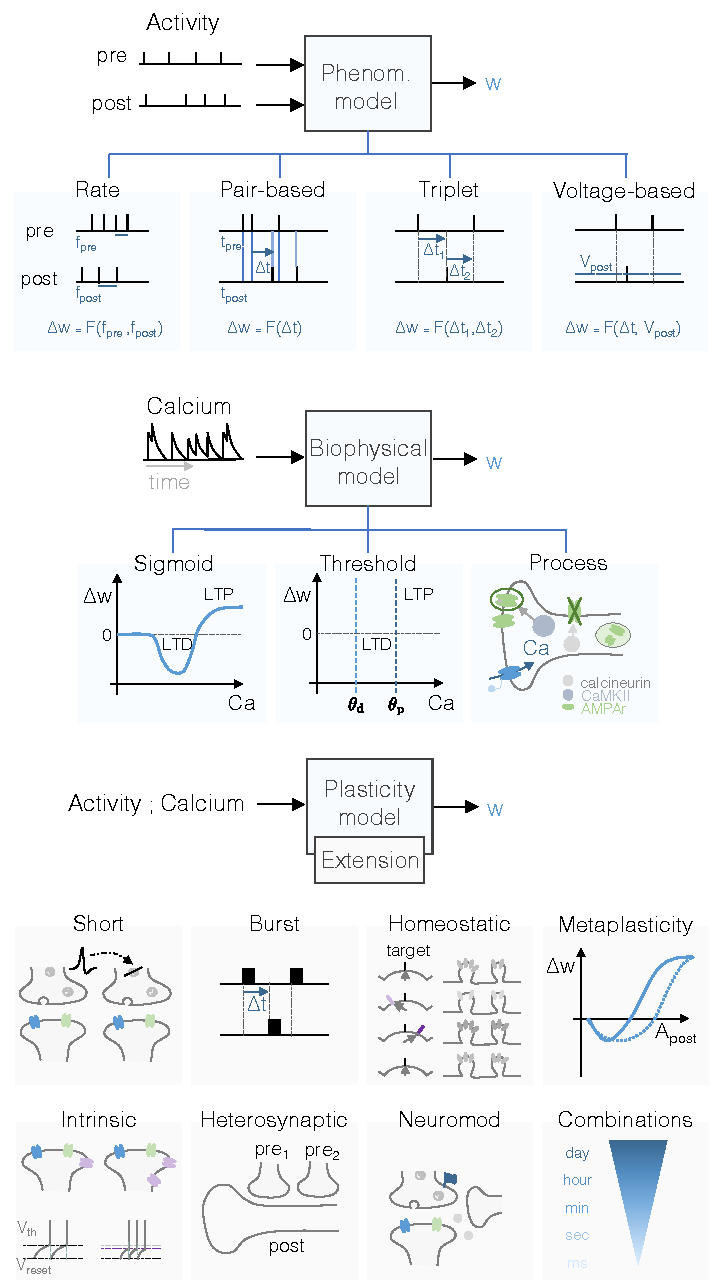
\includegraphics{fig/Review/ModelRecap.pdf}
    \caption{\textbf{Taxonomy of synaptic plasticity rules} . (Top) Phenomenological synaptic plasticity rules compute the synaptic weight change from the pre and post synaptic activities. Four main models are implemented: rate [...], pair-based [...], triplet [...] and voltage-based [...]. (Center) Biophysical models use the calcium signal that drives the synaptic weight change. Three main models exist: sigmoid \citep{shouval_unified_2002}, threshold \citep{graupner_calcium-based_2012} and process encapsulated more complex models [..]. (Bottom) Several extension rules are often encountered: short-term plasticity (short), burst-time dependent plasticity (burst), homeostatic plasticity, metaplasticity, intrinsic plasticity, heterosynaptic plasticity, neuromodulated-plasticity rule (neuromod), combinations of diverse rules. }
    \label{fig:ModelRecap}
\end{figure}
\end{comment}


\subsubsection{Categories of synaptic plasticity rules}
Once the region, the network, the neuron and the definition of the synaptic strength have been established, the next primordial step is the implementation of the synaptic plasticity rule. It is translated by an equation describing the evolution of the weight $w$ throughout time $\dot{w}$. The synaptic rule can be seen as the \textit{black box} converting pre and postsynaptic activity as input ($A_{\mathrm{pre}}$ and $A_{\mathrm{post}}$), which are implemented for example by the spike times, the firing frequency of the pre- and postsynaptic neurons or the calcium concentration and providing the synaptic change as output (see Figure~\ref{fig:Methods_FeaturesRacap}A)  The generic equation is:
$$ \dot{w} = F(A_{\mathrm{pre}}, A_{\mathrm{post}})$$
\textcolor{orange}{(see Figure \ref{fig:blackbox}B)}\\

~\\
Two main categories of synaptic rules are distinguished \citep{shouval_models_2007, graupner_synaptic_2017, clopath_long-term_2019}(see Figure~\ref{fig:Methods_FeaturesRacap}D): 
\begin{itemize}
    \item \textit{Phenomenological models} estimate the synaptic strength change by translating the relationship between neuronal activity and the synaptic plasticity. This category of model expressed mathematically the relation between the pre- and post spike times $(t_{\mathrm{pre}}, t_{\mathrm{post}})$, the firing frequency $(f_{\mathrm{pre}}, f_{\mathrm{post}})$ or the neuronal activity  to estimate the change in synaptic strength. This approach focuses on abstract equations able to fit experimental data rather than describing all molecular processes underneath.
    \item \textit{Biophysical models} using biological variables to drive the induction and expression of synaptic plasticity such as calcium concentration or a cascade of kinase activation for example. Indeed, calcium is a good indicator of voltage, frequency, action potential variation \citep{feldman_spike-timing_2012}.
\end{itemize}

An overview of the most common encountered synaptic plasticity rules is shown in Figure \ref{fig:ModelRecap}. The following sections explained their implementations. This method of classification and model description was started in \citep{clopath_long-term_2019}. 


\subsubsection{Synaptic plasticity rule limitations}
In the context of this thesis, I am restricting my research on excitatory synaptic plasticity and I put aside the inhibitory synaptic plasticity. For more details, refer to \citep{wu_regulation_2022}. Models of plasticity in the field of machine learning and artificial intelligence such as backpropagation for example are out of scope. 

I am interested in articles that investigate the change in synaptic strength due to neuronal activity in order to understand learning, memory formation and memory consolidation. 


\subsubsection{Fitting the parameters of the black box on experimental data}
To create a model, one must choose values for various parameters. To parameterize a synaptic plasticity rule, a common practice is to replicate a plasticity-inducing protocol, as illustrated in Figure \ref{fig:SP_Protocols}. The goal is to fit the experimental points, the two most often encountered dataset is the \acrshort{STDP} provided by \citep{bi_synaptic_1998} (see Figure~\ref{fig:SP_STDP}) or the frequency-dependent plasticity protocol provided by \citep{sjostrom_rate_2001}.


\subsubsection{Phenomenological models}
In phenomenological models, four pioneered synaptic rules were established in the last 20 years: Rate-based, pair-based, triplet and voltage-based as illustrated in Figure \ref{fig:ModelRecap} (top) \citep{gerstner_hebbian_2011, feldman_spike-timing_2012,  feldman_spike_2020}.



In line with the Hebbian principle \citep{hebb_organization_1949}, first models of synaptic plasticity consider only the \textit{rate} of pre- and postsynaptic neurons ($f_{\mathrm{pre}}$, $f_{\mathrm{post}}$) to determine the sign and magnitude of plasticity  [\textcolor{blue}{model:}\cite{oja_simplified_1982, bienenstock_theory_1982, udakis_interneuron-specific_2020}. The \textit{Pair-based} model often called the \textit{\acrfull{STDP}}
[\textcolor{blue}{review}: \cite{abbott_synaptic_2000,morrison_phenomenological_2008})] suggests the equation to fit the experimental data resulting from the plasticity-induction protocol \citep{bi_synaptic_1998}. The pre and the postsynaptic neurons are spiking at  given frequency and the synaptic change depends on the spiking time lag $\Delta t$. It is used in several studies since 20 years [\textcolor{blue}{model}: \cite{van_rossum_stable_2000,song_competitive_2000, capone_sleep-like_2019}. The classical depression-potentiation kernel has been shown to change depending on the region or the animal [\textcolor{blue}{review}: \cite{abbott_synaptic_2000}. It has been exploited for example in \citep{liu_effects_2015} A comprehensive history of STDP is established in [\textcolor{blue}{review}: \cite{markram_history_2011, feldman_spike_2020}. This rule is constrained by some limitations \citep{babadi_stability_2016}. The \textit{triplet} rule considers the effect of spike triplets such as pre-post-pre or post-pre-post [\textcolor{blue}{model}: \cite{froemke_spike-timing-dependent_2002, pfister_triplets_2006, costa_unified_2015, gjorgjieva_triplet_2011}. \textit{Voltage-based} rules take into account the spike-timing in pre- and postsynaptic neurons as well as the membrane voltage of the postsynaptic neurons [\textcolor{blue}{model}: \cite{brader_learning_2007, clopath_connectivity_2010} in order to reproduce a larger variety of experimental protocols \citep{sjostrom_rate_2001, artola_different_1990, nevian_spine_2006}. 
~\\




\begin{figure}[h!]
    \centering
    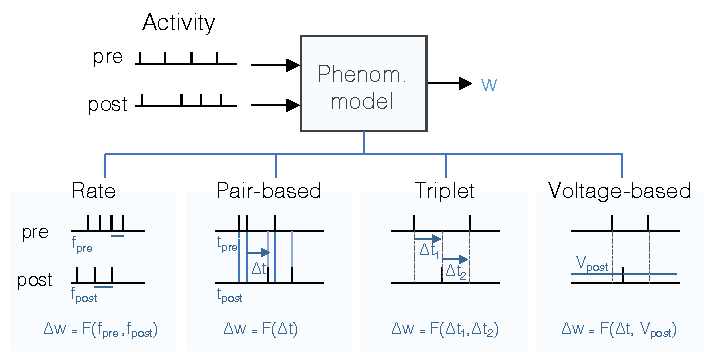
\includegraphics{latex/fig/Methods/ModelRecap_Phenom.pdf}
    \caption{Caption}
    \label{fig:my_label}
\end{figure}


\subsubsection{Calcium-based models}
This part of the review only covers computational models using calcium as the key driver of the synaptic rule. These rules provide equations explaining the calcium influx dependency. Either kinase or phosphatase proteins are activated leading to an increase or decrease of the strength \citep{meriney_synaptic_2019}. This phenomenon is implemented into the synaptic rule with different levels of complexity depending on the model. I highlight three pioneered rules (see Figure \ref{fig:ModelRecap}(center): sigmoid, threshold, and process. 

First, the synaptic change is governed by a \textit{sigmoid} function of the calcium level: $
\tau_w([\mathrm{Ca}]) \dot{w} = \mbox{sig}([\mathrm{Ca}]) - [\mathrm{Ca}] $. It accounts for low calcium level does not change the synaptic weight (or at a extremely slow timescale). Intermediate level triggers slow depression while high calcium level triggers fast potentiation. It reproduces the phosphatase and kinase action. This rule was pioneered by the calcium control hypothesis from \citep{shouval_unified_2002}. The governing rule was further developed throughout time [\textcolor{blue}{model:} \cite{ karmarkar_model_2002, kumar_frequency-dependent_2011, shouval_stochastic_2005, shah_biophysical_2006,cai_effect_2007, carlson_interplay_2011, rackham_ca2-based_2010}. It was used in several applications such as task orientation in place cells or to investigate the effect the dendritic properties
[\textcolor{blue}{model:} \cite{yu_biophysical_2008, iannella_nonlinear_2014, odonnel_dendritic_2011, franks_complexity_2002}. The comparison with phenomeological models such as pair-based on triplet is established in \citep{shouval_what_2011}.


Then, the sigmoid function describing the continuous relationship between calcium concentration and synaptic change was simplified by \citep{graupner_calcium-based_2012} into a two-\textit{thresholds} calcium levels triggering depression and potentiation. The governing expression is $ \tau_w \dot{w} = \gamma_\mathrm{p}(1-w) \Theta([\mathrm{Ca}]-\theta_\mathrm{p}) - \gamma_\mathrm{d} w \Theta([\mathrm{Ca}]-\theta_\mathrm{d})$ where $\tau_w$ is the time constant associated to synaptic change, $\gamma_p$ and  $\gamma_\mathrm{d}$ are respectively the potentiation and the depression rates, $\Theta([\mathrm{Ca}]-\theta_\mathrm{p})$ means $\Theta = 1$ if $[\mathrm{Ca}]>\theta_\mathrm{p}$ otherwise $\Theta = 0$. The comparison with phenomenological models is established in \citep{graupner_natural_2016}. It was used in several studies for various regions such as cerebellum or striatum and diverse applications such as memory formation in large-scale network, \textcolor{blue}{model:} \citep{bouvier_burst-dependent_2016, chindemi_calcium-based_2020, olcese_sleep_2010, standage_calcium-dependent_2014, higgins_memory_2014, inglebert_synaptic_2021, deperrois_short-term_2020,lappalainen_theoretical_2019,jedrzejewska-szmek_calcium_2017}.

A third approach uses intermediate steps that first convert calcium influx into intermediate signals and the change in these signals affect the synaptic weight such as $\dot{w} = F(P),  \dot{P} =F([\mathrm{Ca}])$ where  $P$ quantifies phosphorylation and dephosphorylation processes [\textcolor{blue}{model:} \citep{abarbanel_biophysical_2003, rubin_calcium_2005, badoual_biophysical_2006, hartley_understanding_2006, graupner_stdp_2007, gerkin_phenomenological_2010, bush_calcium_2012, houben_calcium-influx-dependent_2020, kornijcuk_simplified_2020, saudargiene_inhibitory_2015, ebner_unifying_2019}. The level of details in calcium-driven varies a lot and it helps to provide a degree of freedom to explore the effect of biological factors, for example, the contribution of endoplasmic reticulum  \textcolor{blue}{model:} \citep{ kubota_model_2008, urakubo_requirement_2008, mahajan_intracellular_2019}.


This review limits its investigation for articles that are only using a small amount of intermediate signals and excludes papers proposing  detailed mechanisms of the effect of calcium influx on the strength by more intermediates, for example an interesting model is presented in \cite{maki-marttunen_unified_2020, kotaleski_modelling_2010}. Other reviews like \cite{graupner_mechanisms_2010, jaeger_spike_2014} further examine and compare, calcium data, models depending only on calcium concentration, or implement biochemical signaling cascades beyond calcium. 



\begin{figure}[h!]
    \centering
    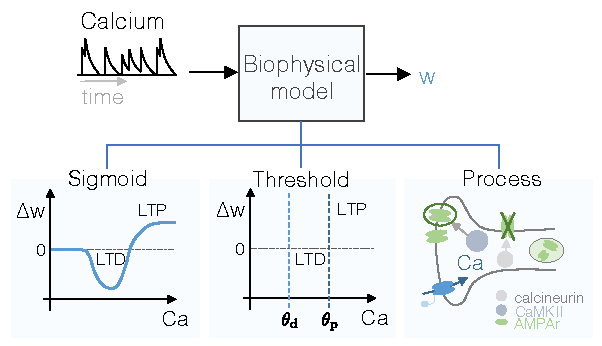
\includegraphics{latex/fig/Methods/ModelRecap_Ca.pdf}
    \caption{Caption}
    \label{fig:my_label}
\end{figure}

\begin{table}[H]
\centering
\begin{small}
\resizebox{\textwidth}{!}{%
\begin{tabular}{llll}
\hline
    Model & Equation &  & Reference  \\
\hline
\multicolumn{4}{c}{\textbf{Phenomenological models}}  \\ 
\hline
    Rate-based & $\dot{w} = F(f_{\mathrm{pre}}, f_{\mathrm{post}})$  &  & \cite{bienenstock_theory_1982}\\
    & & & \cite{oja_simplified_1982}\\
    Pair-based & $\dot{w} = F(\Delta t)=\left\{\begin{array}{ll}A^{+} \exp \left(-\Delta t / \tau^{+}\right) & \Delta t>0 \\- A^{-} \exp (\Delta t / \tau^{-}) & \Delta t<0\end{array}\right.$  &  & \cite{song_competitive_2000}\\
    & & & \cite{van_rossum_stable_2000}\\
    Triplet &  $\dot{w} = F(\Delta t_1, \Delta t_2)$ &   & \cite{pfister_triplets_2006} \\
    Voltage-based & $\dot{w} = F(\Delta t, V_{\mathrm{post}})$ & & \cite{clopath_connectivity_2010}\\
\hline
\multicolumn{4}{c}{\textbf{Biophysical models}}  \\ 
\hline
    Sigmoid   & $\tau_w([\mathrm{Ca}]) \dot{w} = \mathrm{sig}([\mathrm{Ca}]) - [\mathrm{Ca}]$   &  & \cite{shouval_unified_2002} \\
    Threshold &  & & \cite{graupner_calcium-based_2012} \\
    & \begin{tabular}[l]{@{}l@{}} $[\mathrm{Ca}]< \theta_\mathrm{d} :  \dot{w}=0$\\ $\left[\mathrm{Ca} \right] \in \left[\theta_\mathrm{d}, \theta_\mathrm{p} \right] :  \dot{w}=\nearrow$ \\ $\left[\mathrm{Ca} \right] > \theta_\mathrm{p} :  \dot{w} \searrow$ \end{tabular} & & \\
    Process &  \begin{tabular}[l]{@{}l@{}}$\dot{w} = F(P)$ \\ $dP/dt = F([\mathrm{Ca}])$ \end{tabular} &  & \cite{abarbanel_biophysical_2003}\\
\hline
\end{tabular}
}
\end{small}
\caption{Overview of synaptic plasticity rule implementations for phenomenological models or biophysical models. Each category is decomposed into their pioneered rules. Conceptual equations for the synaptic change $\dot{w}$ is provided with a brief description. \textcolor{orange}{Questions: (1)  Ajouter les descriptions ou mettre en caption les symboles $\Delta t$ ? (2) est-ce qu'on cite plusieurs articles par règle ? par exemple pour process il y en a plusieurs ..}}
\label{tab:Phenom}
\end{table}



\subsubsection{Extended models}
The previous synaptic rules are well-known in the literature but it was shown that they cannot explain all the various complex synaptic processes. In this section, we present models describing complementary synaptic mechanisms: (i) short term plasticity, (ii) burst-dependent plasticity, (iii) homeostasis, (iv) metaplasticity, (v) intrinsic plasticity, (vi) heterosynaptic plasticity, (vii) neuromodulated-plasticity and (viii) combinations of synaptic rules. The overview of the extension models are shown in Figure \ref{fig:ModelRecap}(bottom). Table \ref{tab:extensions} briefly presents the implementation of these different extensions and their mechanisms. It extended the work presented in \citep{clopath_long-term_2019}. 

\begin{figure}[h!]
    \centering
    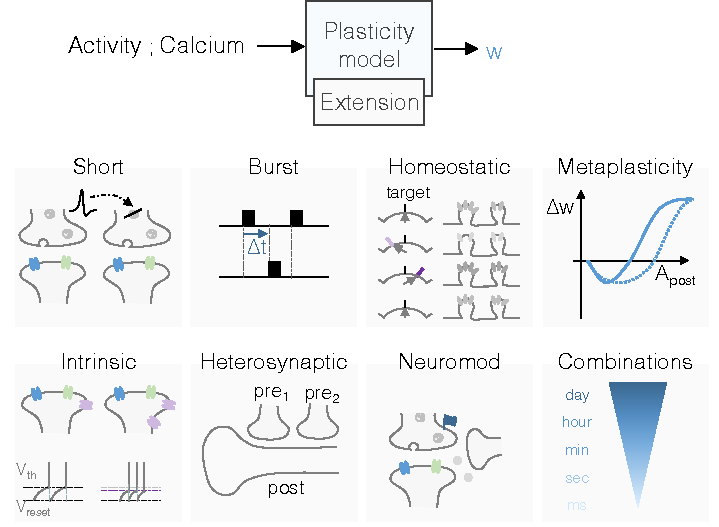
\includegraphics{latex/fig/Methods/ModelRecap_Extension.pdf}
    \caption{Caption}
    \label{fig:my_label}
\end{figure}






(i) \textit{\acrfull{STD}} explains that after an action potential, presynaptic resources such as vesicles transporting neurotransmitters are depleted and need to recover to their initial value before being able to act again [\textcolor{blue}{review/bio:} \cite{zucker_short-term_2002}. It is well known as the Markram-Tsodyks model [\textcolor{blue}{model:} \cite{markram_regulation_1997}. Nowadays, it is common to encountered synaptic plasticity rules including short-term depression in the model [\textcolor{blue}{model:} \cite{zenke_diverse_2015, chen_heterosynaptic_2013, olcese_sleep_2010, shah_biophysical_2006, cai_effect_2007, deperrois_short-term_2020, carvalho_novel_2011, hansel_short-term_2013}. \textcolor{red}{est-ce que je cite uniquement les papiers qui intègrent de la STD ou bien des papiers qui utilisent de la STD avec d'autres combinaisons de règles ? }\\

(ii) The \textit{\acrfull{BTDP}} focuses on the timing of pre- and postsynaptic bursts of activity instead of single-spikes as done in STDP. It permits to integrate the effect of high-frequency burst in the synaptic rule [\textcolor{blue}{model:} \cite{gjorgjieva_burst-time-dependent_2009, delattre_network-timing-dependent_2015, payeur_burst-dependent_2020}.\\


(iii)  Hebbian learning rule often leads to a runaway of synaptic strengths \citep{babadi_stability_2016}. Once the synaptic strengths are modified by a learning rule it can affect the neuronal activity. To counterbalance this problem,  \textit{homeostatic plasticity} refers to compensatory processes operating at various spatial and temporal scales \textit{allowing stabilization of neuronal activity}
[\textcolor{blue}{review:} \cite{turrigiano_homeostatic_2004, karabanov_consensus_2015, meriney_synaptic_2019,desai_homeostatic_2003}. More information on the biological explanations are given in \citep{shepherd_arcarg31_2006}. 

If the target neuronal activity is the firing rate: the concept of homeostatis stands that the connections between neurons should be either scaled up or down respectively as the firing rate decreases or increases [\textcolor{blue}{review} \cite{desai_homeostatic_2016}. In a modeling point of view, this \textit{synaptic scaling} or \textit{normalization} can be implemented via a multiplicative or substractive modifications of the synaptic weights
\citep{oja_simplified_1982}.  If the target neuronal activity is the intracellular calcium level to maintain homeostasis, [\textcolor{blue}{model:} \cite{oleary_cell_2014} developed an homeostatic rule regulating the synaptic conductances as well as the ion channel conductances (see later: intrinsic plasticity). In [\textcolor{blue}{model:} \cite{yeung_synaptic_2004}, the NMDA conductance is regulated leading to regulation of the calcium influx through the NMADr.   \\

(iv) \textit{Metaplasticity} is often called "plasticity of synaptic plasticity" and states that previous activity at the synapse can influence LTP or LTD  [\textcolor{blue}{review:} \cite{ abraham_metaplasticity_1996, abraham_metaplasticity_2008, abraham_is_2019,  meriney_synaptic_2019, deisseroth_synaptic_1995, yger_models_2015, lee_mechanisms_2019}. It can be seen as a modulation of the synaptic rule itself at a larger timescale. In [\textcolor{blue}{model:} \cite{zenke_synaptic_2013, benuskova_stdp_2007}, synaptic rule parameters vary as function of the moving firing rate. Metaplasticity was also investigated in calcium based models [\textcolor{blue}{model:} \cite{yu_biophysical_2008, anirudhan_analogous_2015}.

At this stage, the different terms can be confusing because metaplasticity can be homeostatic or not. If the metaplasticity is homeostatic; the synaptic rule changes itself with the aim of maintaining a target activity \citep{karabanov_consensus_2015}. Metaplasticity that is not homeostatic simply refers to a modification of the synaptic plasticity rule parameters. Similar reasoning, homeostasic plasticity is metaplasticity, if the rule changes or is not metaplastic if different parameters such as the weights are scaled or the intrinsic properties are perturbed. \\

(v) Until now, we have presented plasticity rules that affect the synaptic connection between neurons. However, activity-dependent modification of intrinsic neuronal excitability performed by change of neuronal membrane properties, more specifically  the number, distribution or activity of various ion channels located throughout the neuron  is another mode of memory formation and storage [\textcolor{blue}{review:} \cite{debanne_plasticity_2019, caverzasio_brain_2018, daoudal_long-term_2003, zhang_other_2003, oleary_computational_2015}.  This mode is called \textit{intrinsic plasticity} \citep{titley_toward_2017}. Two of the pioneered papers in this field are \citep{lemasson_activity-dependent_1993, liu_model_1998}.


Once again, intrinsic plasticity can be homeostatic as summarized in [\textcolor{blue}{review:} \cite{williams_homeostatic_2013, turrigiano_hebb_2000} and model in [\textcolor{blue}{model:} \cite{honnuraiah_calcium-dependent_2013, oleary_cell_2014}. Another implementation of intrinsic plasticity in a integrate-and-fire model is achieved by tuning regulating the firing threshold [\textcolor{blue}{model:} \cite{wu_homeostatic_2020}. In rate-based model, intrinsic plasticity tunes the excitability threshold [\textcolor{blue}{model:} \cite{delamare_intrinsic_2022}.  Homeostatic plasticity, intrinsic plasticity and metaplasticity can be hard to identify or separate in some models. The three concepts can be modeled based with concomitant rules. Likewise, one rule can support those concepts as shown in 
[\textcolor{blue}{model:} \cite{sehgal_learning_2013} where the intrinsic plasticity exhibits metaplasticity. \\


%Altogether, intrinsic plasticity and synaptic plasticity can be combined for the benefit of homeostatic regulation of neuronal excitability in order to maintain a target level of electrical activity. In a computational point of view, it can be seen as a controller where the target activity level is the reference such as a given frequency for phenomenological model or calcium level for calcium-based models see later. The intrinsic synaptic rule is the control rule itself transforming the input, ie the activity, into a modification of intrinsic property such as the ion-channel parameters.


(vi) The classical view of synaptic plasticity is built on both presynaptic and postsynaptic neuron activation for plasticity induction.  The rules previously described are input-specific and can be categorized as homosynaptic plasticity. However, at the same postsynaptic neuron, \textit{heterosynaptic plasticity} refers to changes at synapses that are not presynaptically active during the induction protocol, in others words, the synaptic change is induced by activity in neighboring synapses [\textcolor{blue}{review:} \cite{meriney_synaptic_2019, timofeev_sleep-wake_2019}.  Calcium in one synapse can trigger change in the neighboring synapses [\textcolor{blue}{review:} \cite{ bannon_homeostatic_2016, chistiakova_heterosynaptic_2014, froemke_plasticity_2015}. Thus, heterosynaptic plasticity is generated by the same protocols, operates at the same timescale and shares similar mechanisms with homosynaptic plasticity. It offers a solution for competition and stabilization by providing a rapid normalization of synaptic strength over individual cells and multi-cellular networks. In a computational point of view, the synaptic strength is driven as already explained by the pre- and postsynaptic neuronal activity as well as the neighboring activity (phenomenological manner) or by affecting modeling the calcium fluctuation coming from the pre, post and neighboring synapses (biophysical manner)  [\textcolor{blue}{model:} \cite{chen_heterosynaptic_2013, field_heterosynaptic_2020, hiratani_detailed_2017, li_induction_2016, fiete_spike-time-dependent_2010}. \\

(vii) Experimental studies have more recently investigated  the interaction of \textit{neuromodulation} and synaptic plasticity (see [ \textcolor{blue}{bio:} \cite{seol_neuromodulators_2007, zhang_gain_2009, salgado_noradrenergic_2012, pawlak_dopamine_2008, nadim_neuromodulation_2014}). The effect of the different neuromodulators on synaptic plasticity are very complex. To name a few, neuromodulatory inputs gate STDP rules via modification of neuronal excitability and spiking dynamics or alteration of intracellular signaling cascades implied in synaptic
plasticity [ \textcolor{blue}{review:} \cite{brzosko_neuromodulation_2019,fremaux_neuromodulated_2015, pawlak_timing_2010}. There are several ways to derive neuromodulated synaptic plasticity. The first one is inspired by neuromodulated-STDP. While adding neuromodulators during the STDP protocol, the kernel is shifted [\textcolor{blue}{model:} \cite{pedrosa_role_2017, gonzalez-rueda_activity-dependent_2018, izhikevich_solving_2007, legenstein_learning_2008}. Another technique relies on the creation of a mathematical framework called a "\textit{three-factor rule}". Plasticity is driven by the pre- and postsynaptic activity  as well as, a global factor seen as an extrinsic signal since it is not generated itself by the considered neurons but rather by others structures [\textcolor{blue}{review:} \cite{marder_neuromodulation_2012, fremaux_reinforcement_2013, izhikevich_solving_2007, brzosko_neuromodulation_2019, fremaux_neuromodulated_2015,schultz_behavioral_2006, foncelle_modulation_2018}. A synaptic \textit{eligibility trace} $e(t)$ bridges the temporal gap between the neural activity and the neuromodulatory signal. In experimental literature, this  eligibility trace is also called a 'tag'. It means that the synapse is 'tagged' and 'eligible' for change later on \citep{fremaux_neuromodulated_2015, magee_synaptic_2020}. But the synaptic change requires a modulatory signal to be effectively operated. One pays attention to the distinction between the two variables $w$ and $e$. The variable $w$ refers to the synaptic weight. The internal variable $e$ is not measurable in standard electrophysiological experiment \citep{gerstner_eligibility_2018}. More details on the mathematical implementation are available on \cite{izhikevich_solving_2007, legenstein_learning_2008,gerstner_eligibility_2018,fremaux_neuromodulated_2015, pawlak_timing_2010, madadi_asl_dopaminergic_2018}.  

This framework is attractive for reward-based learning, surprise-based learning and novelty-based learning in the sense that the tag exists on the timescale of seconds [\textcolor{blue}{model:} \cite{nakano_kinetic_2010, zannone_acetylcholine-modulated_2018, ang_functional_2021}. In addition, this mathematical formalism is used for memory consolidation and especially for sleep-dependent memory consolidation with the hypothesis called \textit{\acrfull{STD}} [\textcolor{blue}{review:} \cite{seibt_primed_2019}. Indeed, synapses are \textit{tagged} during learning phase and the neuronal network reactivation promotes the \textit{capture} and translation of Plasticity Related Products (PRPs) (including proteins or mRNA synthesis) to engage the pruning or weakening of the tagged synapses [\textcolor{blue}{model} \cite{luboeinski_memory_2021, ziegler_synaptic_2015, clopath_tag-trigger-consolidation_2008, clopath_synaptic_2012}. The website \url{https://www.science.gov/topicpages/r/reward-modulated+spike-timing-dependent+plasticity.html#} gathers numerous models of neuromodulated-synaptic plasticity rules. In brief, the three main modeling strategies of neuromodulated synaptic plasticity are: shifting the STDP kernel by mimicking neuromodulator effects, adding a third-factor term also called eligibility trace or implementing a STC plasticity rule.  \\


(viii) Synaptic plasticity is complex occurring at different places and at different timescales. It is likely that one rule alone is not enough to have the all picture of the different mechanisms. Therefore, several papers \textit{combine different synaptic rules} at different timescales such as STDP, short term plasticity, metaplasticity or homeostasis altogether [\textcolor{blue}{model:} \cite{honnuraiah_calcium-dependent_2013, bannon_adenosine_2017, fauth_self-organized_2019, zenke_diverse_2015, farries_reinforcement_2007, wu_homeostatic_2020,  el_boustani_stable_2012, nere_sleep-dependent_2013, vignoud_interplay_2018}.



\begin{table}[h!]
    \centering
    \resizebox{\textwidth}{!}{%
    \begin{tabular}{llll}
    \hline
    Rule & Equation  &  Description & Reference \\
    \hline
    Short-term &
    & & \cite{zucker_short-term_2002}  \\
    &$\tau_{ST} \dot{X}_{ST} =1-X_{ST}$   &  \begin{tabular}[l]{@{}l@{}} 
    $X_{ST}$: presynaptic resource, \\ $\tau_{ST}$: resource recovery time-constant  \end{tabular} & \cite{zenke_diverse_2015}\\
    \hline
    Burst & $\dot{w} = F(\Delta t^{\mathrm{burst}})$  & $ \Delta t^{\mathrm{burst}}$: relative pre and post synaptic burst timelag & \cite{gjorgjieva_burst-time-dependent_2009} \\
    \hline
    Homeostasis & & & \\
     & scaling: $w = w/w_{\mathrm{max}}$ & $w_{\mathrm{max}}$: maximum weight & \cite{turrigiano_homeostatic_2012} \\
     & target activity: $ \dot{x} \alpha A_{\mathrm{tgt}} - A $ & 
     \begin{tabular}[l]{@{}l@{}} 
     $x$ : weight or ionic conductance\\
     $A_{\mathrm{tgt}}$: target activity \\
    $A$: current activity  \end{tabular}
    & \cite{williams_homeostatic_2013}\\
    & & & \cite{desai_homeostatic_2016}\\
    \hline 
    Metaplasticity & 
    \begin{tabular}[l]{@{}l@{}} 
    $\tau_w \dot{w} = F(\theta)$\\
   $\tau_\theta \dot{\theta} = F(A_{\mathrm{post}})$
    \end{tabular}
    &
    \begin{tabular}[l]{@{}l@{}} 
    $\theta$: ...\\
   $A_{\mathrm{post}}$: ...
    \end{tabular}
    & \cite{abraham_metaplasticity_1996} \\
    \hline
    Intrinsic & \begin{tabular}[l]{@{}l@{}} $\dot{g}_{\mathrm{ion}} = F(A)$ \\ $g_{\mathrm{ion}}$: neuron-related variable \\
    (ion channel conductance, excitability,...)\\
    $A$: neuronal activity 
    \end{tabular} & & ... \\
    \hline
    Heterosynaptic & $\dot{w_{kj}} = F(A_i,A_j, A_k)$ &
    \begin{tabular}[l]{@{}l@{}}
    $A_{i,j}$: activity of presynaptic neuron i or j\\
    $A_{k}$: activity of postsynaptic neuron k\\    
    Activity is can be spike times or calcium concentration
    \end{tabular} &  \cite{chen_heterosynaptic_2013}\\
    & & & \cite{field_heterosynaptic_2020}\\
    \hline
    Neuromodulated & STDP kernel shift &
    & \cite{pedrosa_role_2017} \\
    &eligibility trace     &  & \cite{foncelle_modulation_2018}\\
    & STC   & & \cite{clopath_tag-trigger-consolidation_2008}\\
    & \begin{tabular}[l]{@{}l@{}}
    $\dot{w} = F(A_{\mathrm{pre}}, A_{\mathrm{post}}, M)$\\
    $M$: Neuromodulator variable
    \end{tabular}  & &\\
    \hline
    Combination & $\dot{w} = F(\mathrm{rule}_1, \mathrm{rule}_2)$ & Combinations of different synaptic rules at different timescales & \cite{zenke_diverse_2015}\\
    & & &\cite{fauth_self-organized_2019}\\
    & & & ... \\
    \hline
    \end{tabular}
    }
    \caption{Extensions of synaptic plasticity rules. Each rule is described with a conceptual equation / mathematical framework. }
    \label{tab:extensions}
\end{table}



% ---------------------------------------------
% ---------------------------------------------
%
%       TAXONOMY >> aboutir aux excels 
%
% ---------------------------------------------
% ---------------------------------------------

\subsection{Taxonomy of synaptic plasticity rules}
Putting into equation the famous quote "Fire together, wire together" is a significant challenge, as confirmed by the numerous models used to explore learning, memory formation and consolidation, and to detail plasticity biophysical mechanisms in order to better understand the signaling cascade. With the abundance of scientific articles available, it can be a daunting task to determine whether a proposed synaptic rule can be applied to a particular problem. This raises several questions, such as how to model neurons and which category of rules should be employed.

To facilitate the search for information, I have created a taxonomy of articles investigating synaptic plasticity rules described in the past 25 years in a systematic manner. The objective of this review is to \textit{classify} the existing models based on their rules and their computational features or model practices. This non-exhaustive classification as been 

The Excel sheets contain a non-exhaustive list of the different synaptic rules found in the literature. These rules are classified according to the presented features.




\begin{table}[h!]
\begin{flushleft}
A. Model features\\
\end{flushleft}
    \centering
        \resizebox{\textwidth}{!}{%
\begin{tabular}{|l| l | l| l|}
\hline
    Region & Network size & Neuron model & Synaptic strength   \\
    \hline
    Hippocampus (H) & One postsynaptic neuron (1) &  Conductance-based (cond) & Abstract weight (abstract) \\
    Cortex (C) & One pre- to one postsynaptic neuron (1-1) & Integrate-and-Fire (IF) & Weighted synaptic input (Isyn) \\
    Striatum (S) & Several pre to one postsynaptic neuron (L-1) & Event-based implementation (EB) & AMPA conductance (AMPA) \\
    Thalamus (T) & Network/memory assembly (Network) & Rate-based (rate) &  Change in EPSP (EPSP) \\
    Adaptable neuron parameters (adaptable) & & EPSP, BPAP, ... (Others) & Biological description (bio) \\
    Abstract neuron (abstract) & & & \\
\hline
\end{tabular}
}
~\\
\begin{flushleft}
B. Synaptic plasticity rules\\
\end{flushleft}
\resizebox{10cm}{!}{%
\begin{tabular}{|l||l||l|}
\hline
    Phenomenological rule &  Calcium-based rule & Extended plasticity ryle \\
    \hline
    Rate & Sigmoid  & Short-term \\
    Spike-Time  & Threshold & Burst-dependent\\
    Triplet     & Process & Homeostatic \\
    Voltage-dependent &  & Metaplasticity \\
    & & Intrinsic \\
    & & Heterosynaptic \\
    & & Neuromodulated\\
    & & Combinations \\
    \hline
\end{tabular}
}
    \caption{\textbf{Criteria for the taxonomy of synaptic plasticity rules}. A. Classification of model features shared in computational models of synaptic plasticity. The label in brackets are found in the excel sheet. B. Classification of synaptic plasticity rules.  \textcolor{red}{diviser le tableau en 2}}
    \label{tab:Review_features}
\end{table}



\subsection{Implementation of the synaptic plasticity rules in the context of this thesis}
\subsubsection{Pair-based model}

\subsubsection{Triplet model}

\subsubsection{Calcium-based}

\textcolor{red}{faire les simu ici }


\subsection{Structural synaptic plasticity rules}



\newpage



% -----------------------------------
% -----------------------------------
%
%       Measures with equations
%
% -----------------------------------
% -----------------------------------
\section{Mesures et analyses (LFP, Spectrogram)}
The local field potential measures the average behavior of interacting neurons \cite{drion_cellular_2019, jacquerie_robust_2021, jacquerie_switches_2022}. It reflects the collective synaptic activity in a neuron population. In the situation 2-layer feedforward network with 10 presynaptic neurons connected to 3 postsynaptic neurons through AMPA receptors, the postsynaptic current computed at the postsynaptic neuron $j$ from the presynaptic neuron $i$ is $$I_{\mathrm{syn},ij}(t) = -\bar{g}_{\mathrm{AMPA},ij} s_{\mathrm{AMPA},ij} (V_j - 0).$$
The negative sign is a convention coming from the equivalent circuit modeling.  The total synaptic current at the postsynaptic neuron $j$ is the average sum over all the input current driven by the 10 presynaptic neurons: 
$$ I_{\mathrm{syn},j}(t) = \frac{1}{10} \sum_{i=1}^{10} I_{\mathrm{syn},ij}(t) $$
Finally, the overall synaptic activity is given by the mean of all the postsynaptic neurons: 
$$ \mathrm{LFP}(t) = \kappa \frac{1}{3} \sum_{j=1}^3 I_{\mathrm{syn},j}(t)$$
$\kappa$ is a current-to-voltage factor to respect unit. In this thesis, it is equal to 1 because \textcolor{orange}{QUESTION POUR GD > meme dans l'article du reset parce que c'est normalement en $\mu V$}

Then, the \acrshort{LFP} signal is filtered by a butterworth filter at a cutoff frequency equal to 100Hz - reflecting the use of macro-electrodes in LFP acquisition. 

\acrshort{LFP} is a valuable tool to explore the fluctuation in brain activity. I quantify the LFP by displaying the time-frequency evolution, namely creating the spectrogram. 


\citep{esser_breakdown_2009, mazzoni_computing_2015, telenczuk_kernel-based_2020}